On considère un pavé droit $ABCDA'B'C'D'$ avec $DD'= 5$ cm ; $DC= 6$ cm et $DA = 7$ cm.

On note L le point d’intersection des diagonales $[AC]$ et $[BD]$.

On souhaite creuser ce pavé, en retirant une pyramide $OABCD$ de hauteur $[OL]$.


\begin{center}
	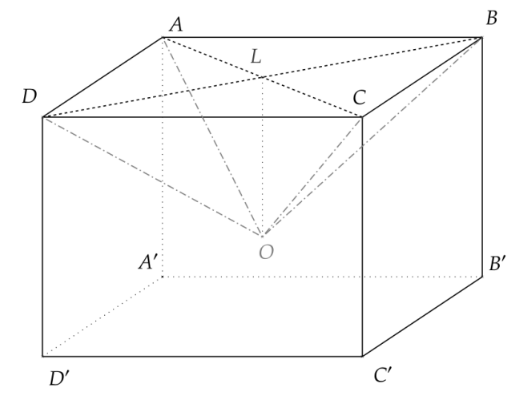
\includegraphics[width=.5\textwidth]{./images/2022-g2-ex3-img1.png}
\end{center}

\subsection*{Partie A}
Dans cette partie, on suppose que $OL=4$ cm.
\begin{enumerate}
\item Montrer que $AL\approx4,6$ cm.
\item Construire le triangle $ALO$ en vraie grandeur.
\item 
\begin{enumerate}
	\item Calculer le volume de la pyramide $OABCD$.
	
\textit{On rappelle que le volume d’une pyramide est égal au tiers du produit de l’aire de sa base par sa hauteur.}

\item Calculer le volume du pavé creusé.
\end{enumerate}
\end{enumerate}

\subsection*{Partie B}

\begin{minipage}{12cm}
Dans cette partie, on pose $OL = x$, où $x$ est un nombre compris entre 0 et 5. Le pavé creusé que l’on
obtient est le socle en bois d'un trophée. Sur ce socle, on pose une pyramide en verre $OEFGH$ qui est
un agrandissement de la pyramide $OABCD$ de rapport 2.
\end{minipage}
\begin{minipage}{7cm}
\begin{center}
	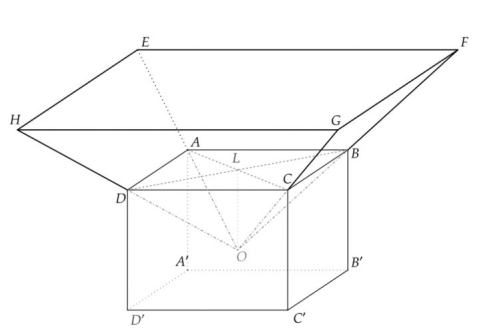
\includegraphics[width=.9\textwidth]{./images/2022-g2-ex3-img2.png}
\end{center}
\end{minipage}

\begin{enumerate}
\item Exprimer le volume de la pyramide $OABCD$ en fonction de $x$.
\item Montrer que le volume du socle en bois est $210 - 14x$.
\item Montrer que le volume de la pyramide en verre $OEFGH$ est $112x$.
\item Quelle valeur choisir pour $x$, pour que le volume de la pyramide en verre soit égal au
double du volume du socle en bois ?
\item On considère les fonctions $f$ et $g$ définies pour tout $x$ compris entre 0 et 5 par :

$$f(x) = 210 – 14x ~\text{et}~ g(x) = 112x$$

On a représenté dans un repère orthogonal ces deux fonctions.
\begin{center}
	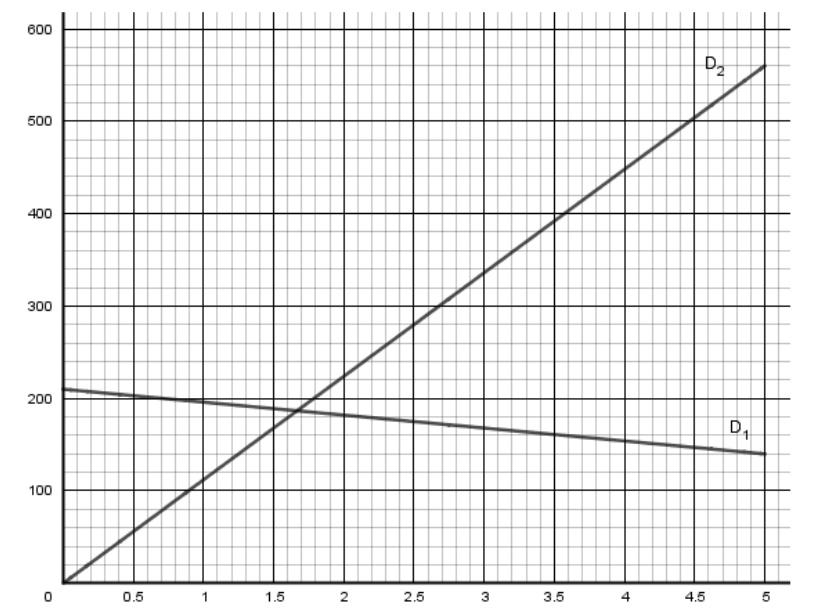
\includegraphics[width=.8\textwidth]{./images/2022-g2-ex3-img3.png}
\end{center}
\begin{enumerate}
	\item Déterminer quelle fonction ($f$ ou $g$) est représentée par chacune des droites $D_1$ et
$D_2$ ? Justifier.
	\item Déterminer avec la précision permise par le graphique les valeurs de $x$ pour
lesquelles le volume du socle en bois est inférieur ou égal au volume de la pyramide en verre.
	\item Retrouver le résultat précédent en posant puis en résolvant une inéquation.
\end{enumerate}
\end{enumerate}